\documentclass{standalone}

\usepackage{pgfplots}
\pgfplotsset{compat=1.12}

\begin{document}

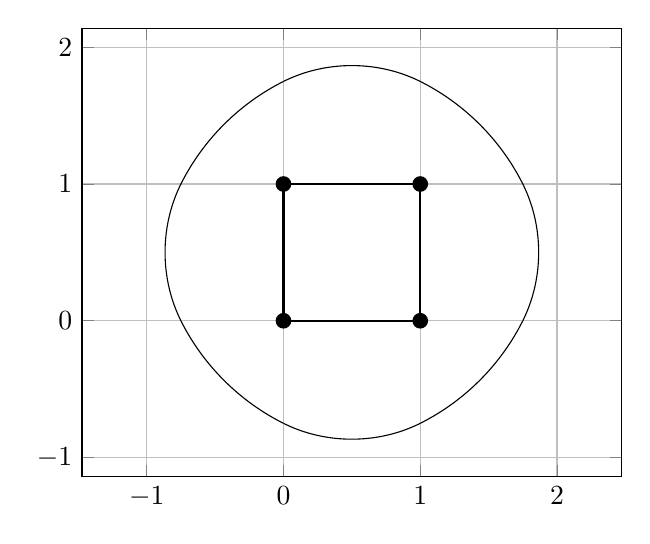
\begin{tikzpicture}
\begin{axis}[grid=both,trig format plots=rad, axis equal]
\draw[thick] (0.0, 0.0)
-- (1.0, 0.0)
-- (1.0, 1.0)
-- (0.0, 1.0)
-- cycle;
\node [circle, fill=black, inner sep=2pt] at (0.0, 0.0) {};
\node [circle, fill=black, inner sep=2pt] at (1.0, 0.0) {};
\node [circle, fill=black, inner sep=2pt] at (1.0, 1.0) {};
\node [circle, fill=black, inner sep=2pt] at (0.0, 1.0) {};

\addplot [domain=1.04719755:2.09439510,samples=50]({0.50000000 + -1.00000000*cos(\x) + -0.00000000 * sin(\x)},{0.00000000 + 0.00000000*cos(\x) + -0.86602540 * sin(\x)}); 
\addplot [domain=1.20942920:1.93216345,samples=50]({0.50000000 + -1.06066017*cos(\x) + 0.93541435 * sin(\x)},{0.50000000 + -1.06066017*cos(\x) + -0.93541435 * sin(\x)}); 
\addplot [domain=1.04719755:2.09439510,samples=50]({1.00000000 + 0.00000000*cos(\x) + 0.86602540 * sin(\x)},{0.50000000 + -1.00000000*cos(\x) + 0.00000000 * sin(\x)}); 
\addplot [domain=1.20942920:1.93216345,samples=50]({0.50000000 + 1.06066017*cos(\x) + 0.93541435 * sin(\x)},{0.50000000 + -1.06066017*cos(\x) + 0.93541435 * sin(\x)}); 
\addplot [domain=1.04719755:2.09439510,samples=50]({0.50000000 + 1.00000000*cos(\x) + -0.00000000 * sin(\x)},{1.00000000 + 0.00000000*cos(\x) + 0.86602540 * sin(\x)}); 
\addplot [domain=1.20942920:1.93216345,samples=50]({0.50000000 + 1.06066017*cos(\x) + -0.93541435 * sin(\x)},{0.50000000 + 1.06066017*cos(\x) + 0.93541435 * sin(\x)}); 
\addplot [domain=1.04719755:2.09439510,samples=50]({0.00000000 + 0.00000000*cos(\x) + -0.86602540 * sin(\x)},{0.50000000 + 1.00000000*cos(\x) + 0.00000000 * sin(\x)}); 
\addplot [domain=1.20942920:1.93216345,samples=50]({0.50000000 + -1.06066017*cos(\x) + -0.93541435 * sin(\x)},{0.50000000 + 1.06066017*cos(\x) + -0.93541435 * sin(\x)}); 
\end{axis}
\end{tikzpicture}
\end{document}